\documentclass{beamer}
%\setbeamertemplate{background canvas}[vertical
%shading][bottom=green!10,top=blue!10]
%\usetheme{PaloAlto}
\usetheme{classic}
\colorlet{structure}{magenta}
%I found Antibes, Warsaw, Darmstadt
%\usecolortheme{dolphin}
\usepackage{times}
\usefonttheme{structurebold}
\usepackage[english]{babel}
\usepackage{pgf,pgfarrows,pgfnodes,pgfautomata,pgfheaps}
\usepackage{amsmath,amssymb}
\usepackage[latin1]{inputenc}
\usepackage{amsmath}
\setbeamercovered{dynamic}
\usepackage{float} %NO SE PARA QUE SE USA
\usepackage{multirow} %NO SE PARA QUE SE USA
\usepackage{psfrag}
\usepackage{enumerate}


% MATH -----------------------------------------------------------
\newcommand{\norm}[1]{\left\Vert#1\right\Vert}
\newcommand{\abs}[1]{\left\vert#1\right\vert}
\newcommand{\set}[1]{\left\{#1\right\}}
\newcommand{\R}{\mathbb R}
\newcommand{\eps}{\varepsilon}
\newcommand{\To}{\longrightarrow}
\newcommand{\BX}{\mathbf{B}(X)}
\newcommand{\Ss}{\mathcal{S}}

%%% --------------------------------------------------------------
\begin{document}
% ----------------------------------------------------------------
\title{Bounding Diameters of Covering Spaces}
\author{Sergio Zamora}
\institute{Penn State University}
\date{Geometry Luncheon Seminar}

\maketitle

%-------------------------------------------------------------------
\begin{frame}\frametitle{}

Let $(X,d)$ be a compact metric space, and $\pi\colon \hat{X} \rightarrow X$ an $m$-fold covering map.
\bigskip

Is there a natural way to lift the metric $d$ to a metric $\hat{d}$ in $\hat{X}$ such that $\pi \colon  (\hat{X}, \hat{d}) \rightarrow (X,d)$ is a local isometry?
\bigskip
\pause

We say that $(X,d)$ is a \textit{length space} if 

$$d(p,q )  =  \inf \{  \ell (\gamma) \mid \gamma \colon [0,1] \rightarrow X , \gamma(0)=p, \gamma(1)=q   \}.$$

If $(X,d)$ is a length space, we can define the metric $\hat{d}$ on $\hat{X}$ as

$$ \hat{d}(x,y)   =  \inf \{ \ell (\pi \circ \gamma) \mid   \gamma : [0,1] , \gamma(0)=x , \gamma(1) =y     \}.   $$


\end{frame}


%-------------------------------------------------------


\begin{frame}\frametitle{}


\begin{block}{Main Problem}
{Estimate $diam(\hat{X}) $ in terms of $X$ and the number of sheets.
}
\end{block}
\bigskip


Since $\hat{X}$ as a set is $m$ copies of $X$ one may expect the equality $diam(\hat{X}) = m * diam (X) $, but it is false.

\begin{figure}
\centering
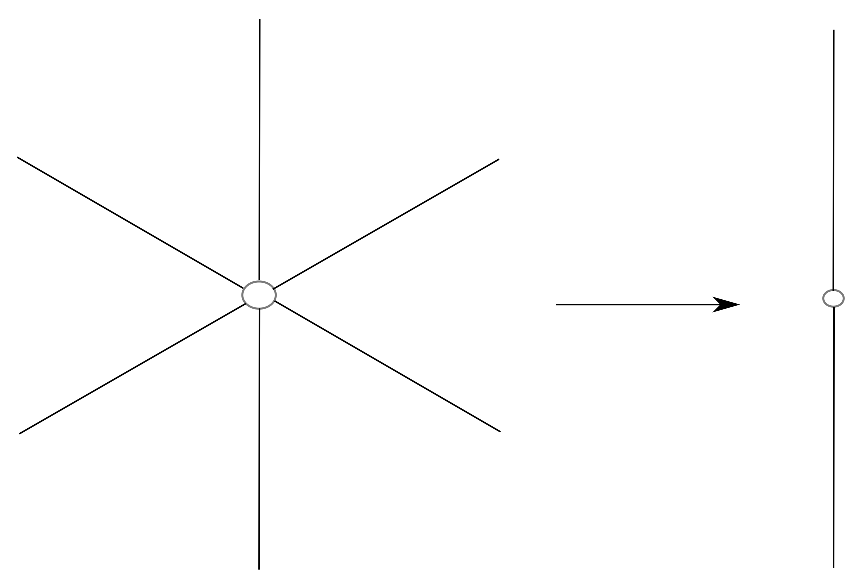
\includegraphics[scale=0.30]{Star.eps}
\end{figure}


If we re-scale $X$, then $\hat{X}$ will suffer the same transformation. So we may assume that $diam(X) = 1$.


\end{frame}

%--------------------------------------------------------------------






\begin{frame}\frametitle{}

\begin{block}{Theorem (Ivanov, 2010)}
{Let $\hat{X}$ be the $m$ fold covering of a compact length space $X$. If we equip $\hat{X}$ with the lifted metric, then

$$diam (\hat{X})  \leq m. $$

This bound is sharp.
}
\end{block}

\bigskip
\pause
\begin{block}{Conjecture (Petrunin, 2009)}
{If $\hat{X}$ is the $m$-fold universal cover, and $\alpha >0$,

\begin{center}
  $diam(\hat{X}) =   o( m^{\alpha}) $
\end{center}
 as $m \rightarrow \infty$. 
 }
\end{block}


\end{frame}


%----------------------------------------------------------------



\begin{frame}\frametitle{}

Universal Covers look like Cayley graphs of Fundamental Groups.


\begin{figure}
\centering
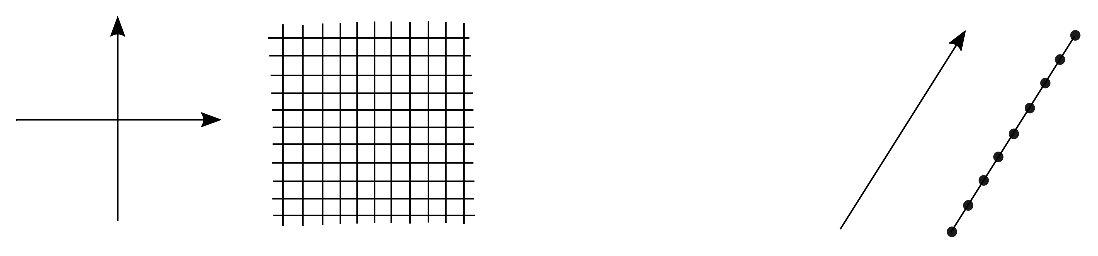
\includegraphics[scale=0.4]{Torus.eps}
\end{figure}

\begin{figure}
\centering
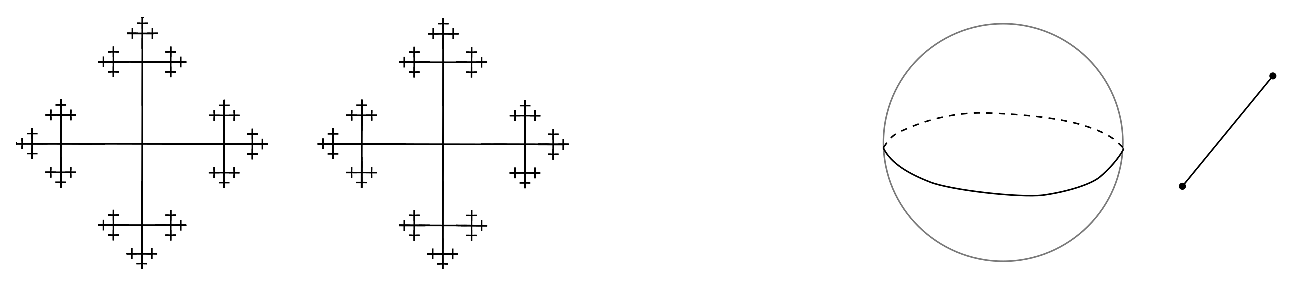
\includegraphics[scale=0.4]{Unicayley.eps}
\end{figure}

\end{frame}

%--------------------------------------------------------------------



\begin{frame}\frametitle{}

\begin{figure}
\centering
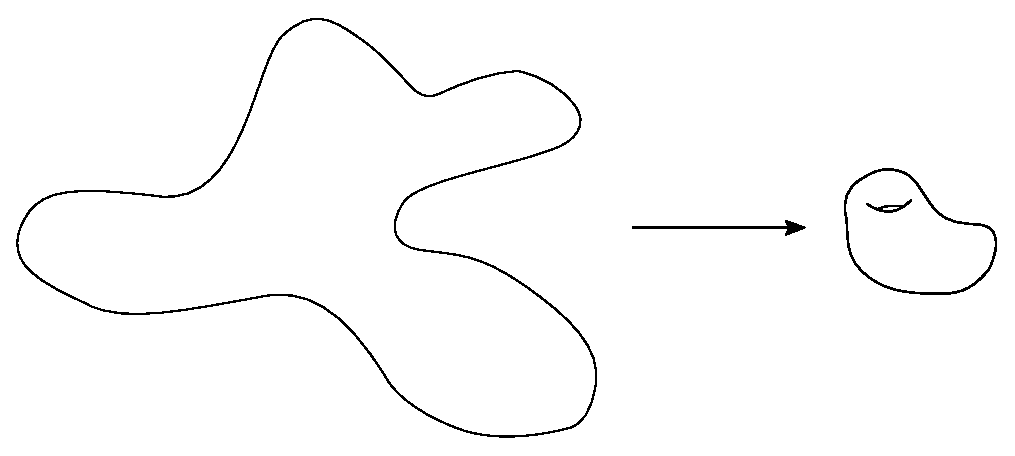
\includegraphics[scale=0.6]{Nerving1.eps}
\end{figure}


\end{frame}
%-------------------------------------------------------------------------



\begin{frame}\frametitle{}

\begin{figure}
\centering
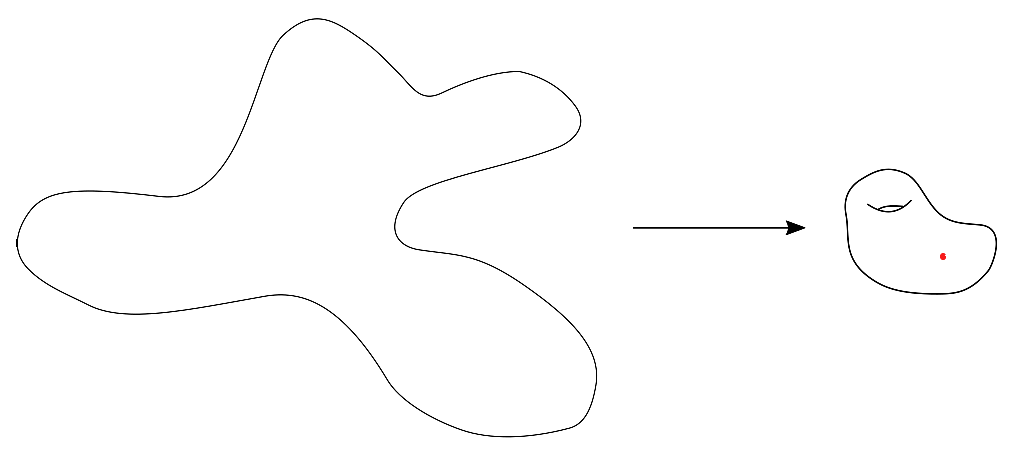
\includegraphics[scale=0.6]{Nerving2.eps}
\end{figure}


\end{frame}
%-------------------------------------------------------------------------


\begin{frame}\frametitle{}

\begin{figure}
\centering
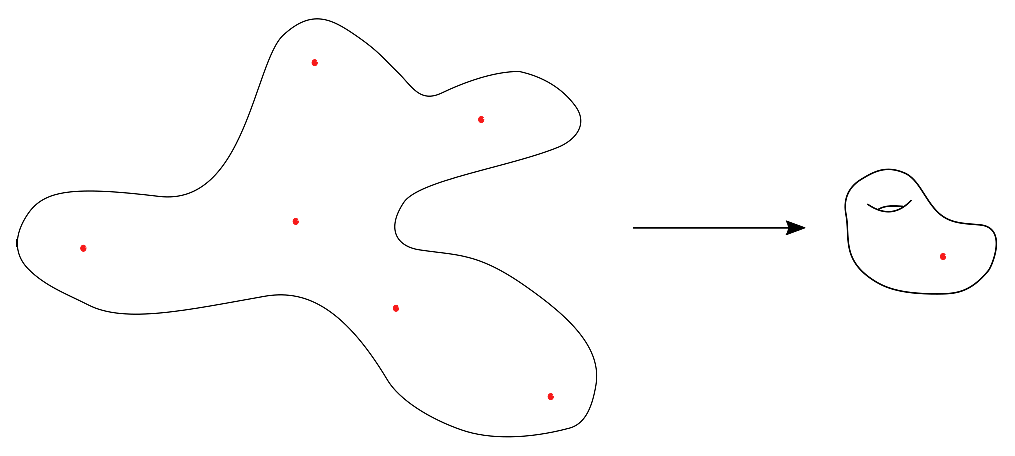
\includegraphics[scale=0.6]{Nerving3.eps}
\end{figure}


\end{frame}
%-------------------------------------------------------------------------


\begin{frame}\frametitle{}

\begin{figure}
\centering
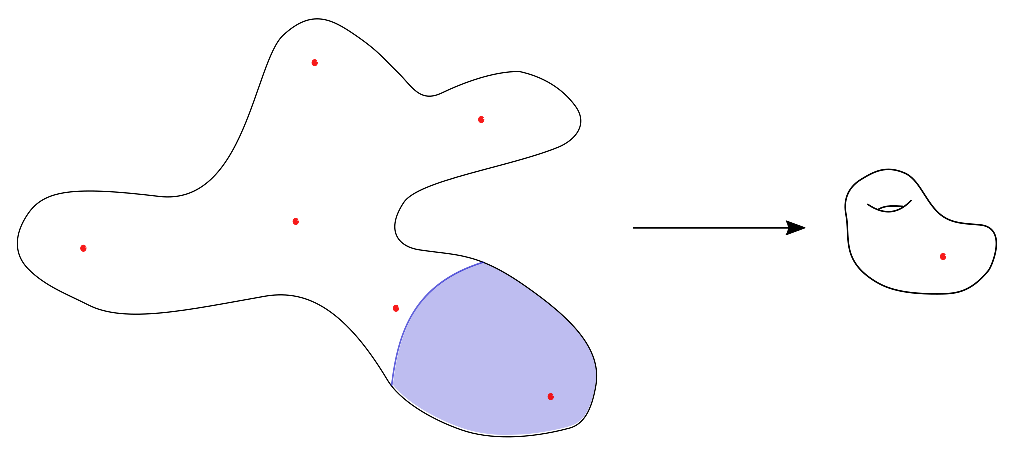
\includegraphics[scale=0.6]{Nerving4.eps}
\caption{We obtain an open cover of balls $\{ B_i \}_{i=1}^m$ of radii $1+\varepsilon$.}
\end{figure}


\end{frame}
%-------------------------------------------------------------------------


\begin{frame}\frametitle{}

\begin{figure}
\centering
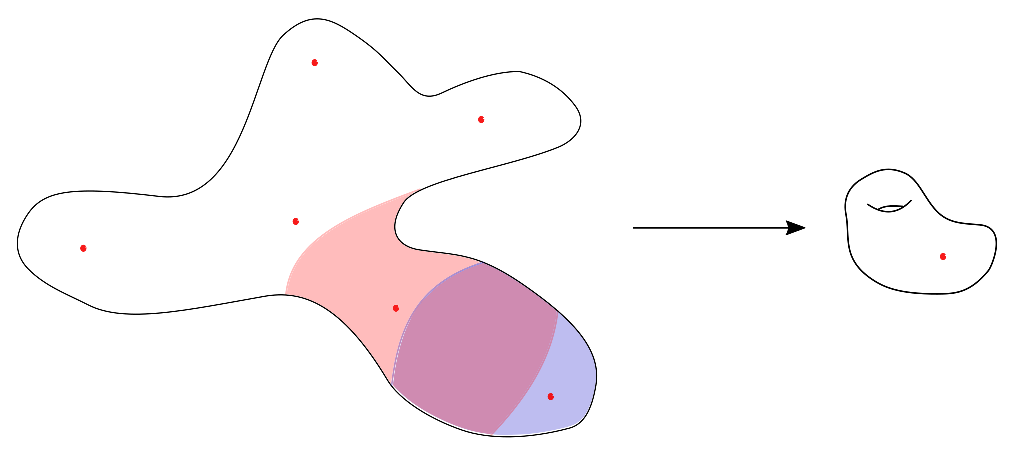
\includegraphics[scale=0.6]{Nerving5.eps}
\caption{We obtain an open cover of balls $\{ B_i \}_{i=1}^m$ of radii $1+\varepsilon$.}
\end{figure}


\end{frame}
%-------------------------------------------------------------------------



\begin{frame}\frametitle{}

\begin{figure}
\centering
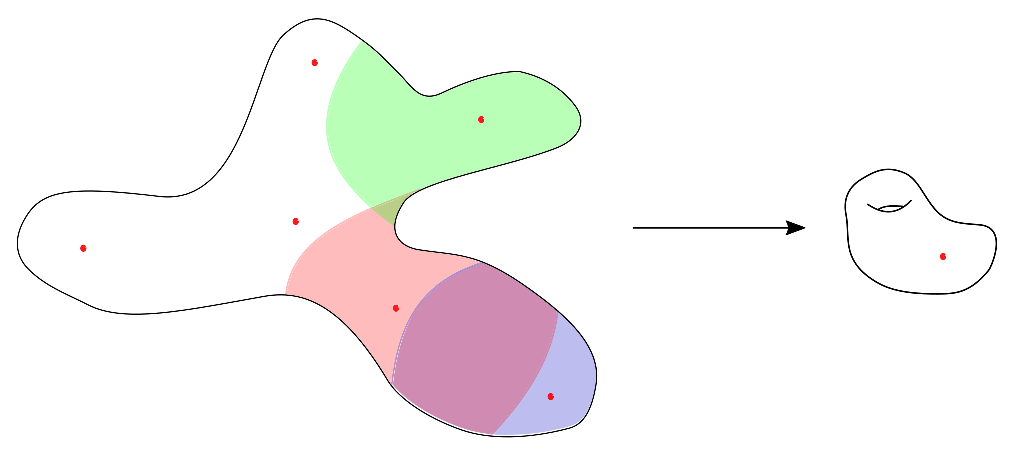
\includegraphics[scale=0.6]{Nerving6.eps}
\caption{We obtain an open cover of balls $\{ B_i \}_{i=1}^m$ of radii $1+\varepsilon$.}
\end{figure}


\end{frame}
%-------------------------------------------------------------------------



\begin{frame}\frametitle{}

\begin{figure}
\centering
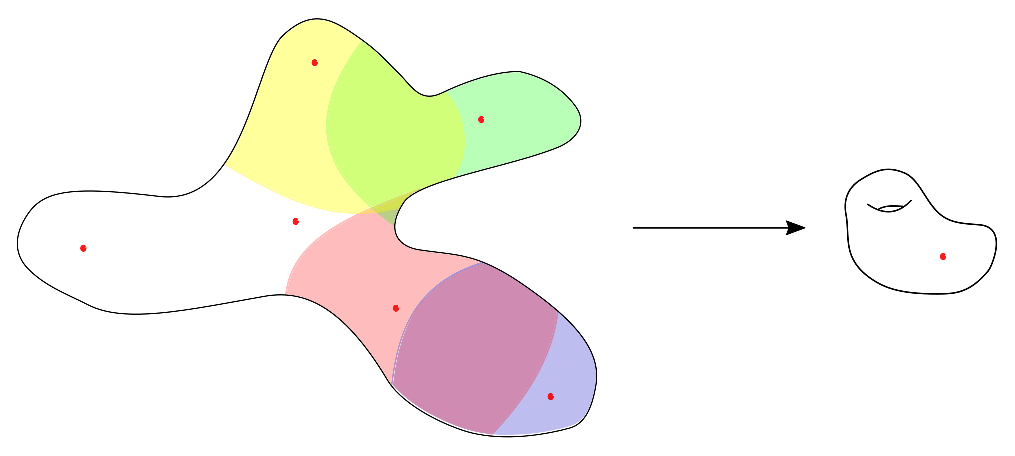
\includegraphics[scale=0.6]{Nerving7.eps}
\caption{We obtain an open cover of balls $\{ B_i \}_{i=1}^m$ of radii $1+\varepsilon$.}
\end{figure}


\end{frame}
%-------------------------------------------------------------------------


\begin{frame}\frametitle{}

\begin{figure}
\centering
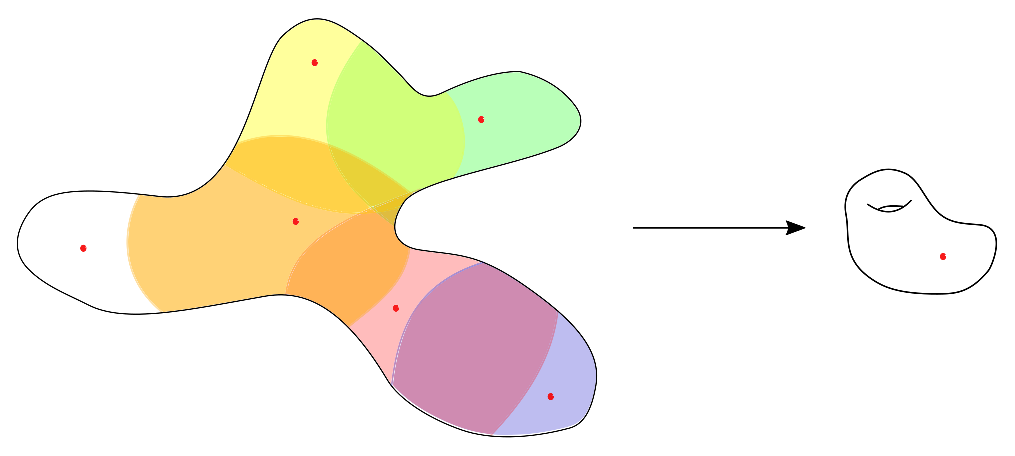
\includegraphics[scale=0.6]{Nerving8.eps}
\caption{We obtain an open cover of balls $\{ B_i \}_{i=1}^m$ of radii $1+\varepsilon$.}
\end{figure}


\end{frame}
%-------------------------------------------------------------------------


\begin{frame}\frametitle{}

\begin{figure}
\centering
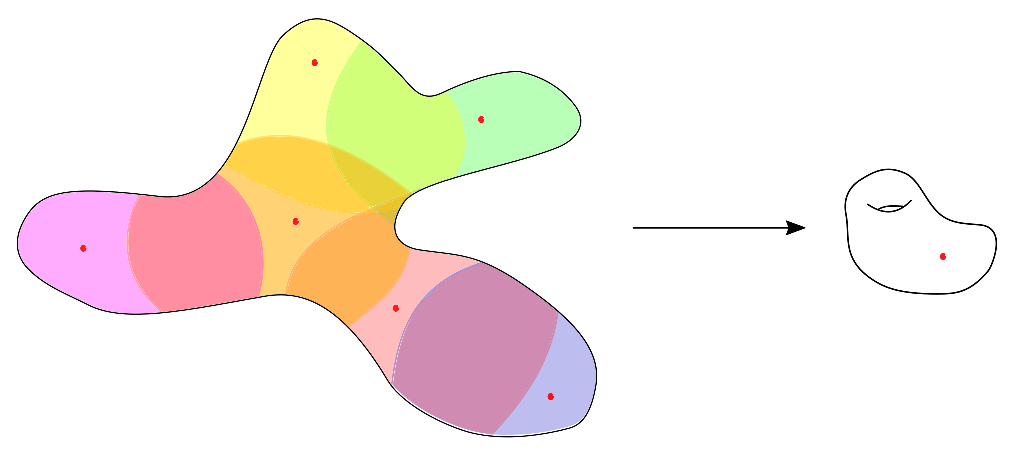
\includegraphics[scale=0.6]{Nerving9.eps}
\caption{We obtain an open cover of balls $\{ B_i \}_{i=1}^m$ of radii $1+\varepsilon$.}
\end{figure}


\end{frame}
%-------------------------------------------------------------------------


\begin{frame}\frametitle{}


The \textit{nerve} of an open cover $\{ U_i \}_{i=1}^m$ is the simplicial complex $ N \leq \Delta^{m-1} \subset \mathbb{R}^m $ with the property that a $k$-dimensional face $  Conv (e_{i_0}, \ldots , e_{i_k}) $ is in $N$ if and only if $U_{i_0}\cap \ldots \cap U_{i_k} \neq \phi$.



\begin{figure}
\centering
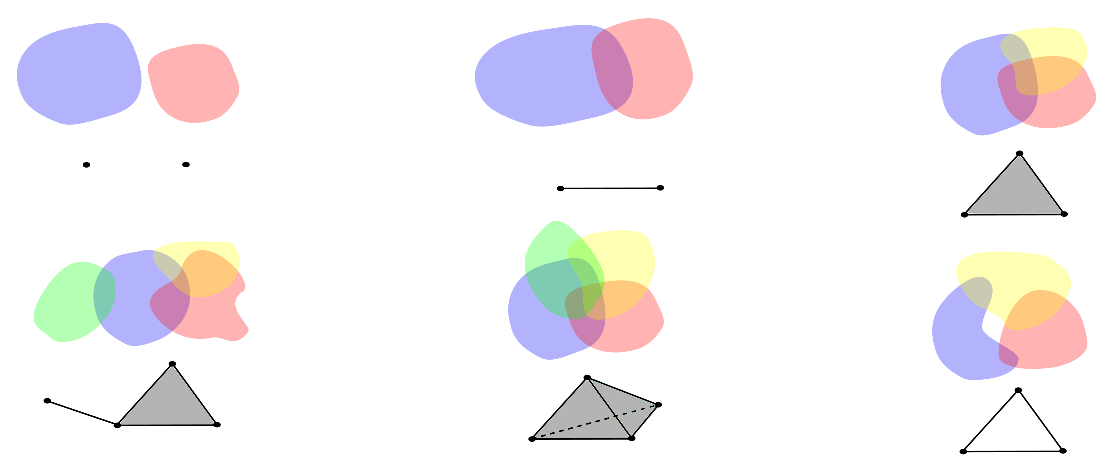
\includegraphics[scale=0.5]{Nerved.eps}
\end{figure}

\pause


The 1-skeleton $N_1$ of the nerve associated to the cover $\{ B_i\}_{i=1}^m$ is the Cayley graph of the fundamental group $\pi_1(X,p)$ with generators the classes with loops of length less than $2+2\varepsilon$. \pause Then $diam(\hat{X}) \leq (2+2\varepsilon)(diam(N_1)+1)$.




\end{frame}
%-------------------------------------------------------------------------


\begin{frame}\frametitle{}

Associated to the cover $\{ B_i \}_{i=1}^m$, we have a partition of unity $\{ f_i  \colon \hat{X} \rightarrow \mathbb{R} \}_{i=1}^m $ with $f_i (x) \neq 0 $ if and only if $x \in B_i$.

\bigskip
\pause

\begin{block}{Nerve Lemma}
{The map $F \colon \hat{X} \rightarrow N \subset \mathbb{R}^m$ given by 
$$ F(x) = (f_1(x), \ldots , f_m(x)) $$
 induces an isomorphism of fundamental groups. In particular, $N$ is simply connected.
 }
\end{block}
\bigskip

\pause

Since the inclusion of the 2-skeleton $i \colon N_2 \rightarrow N$ induces an isomorphism $i_{\ast}\colon \pi_1( N_2) \rightarrow \pi_1( N)$, $N_2$ is simply connected.  


\end{frame}
%-------------------------------------------------------------------------



\begin{frame}\frametitle{}

Then $N_1$ is the 1-skeleton of a 2-dimensional simply connected simplicial complex. That means we can ``patch'' each hole with triangles. We call this the \textit{triangle patch property}.


\begin{figure}
\centering
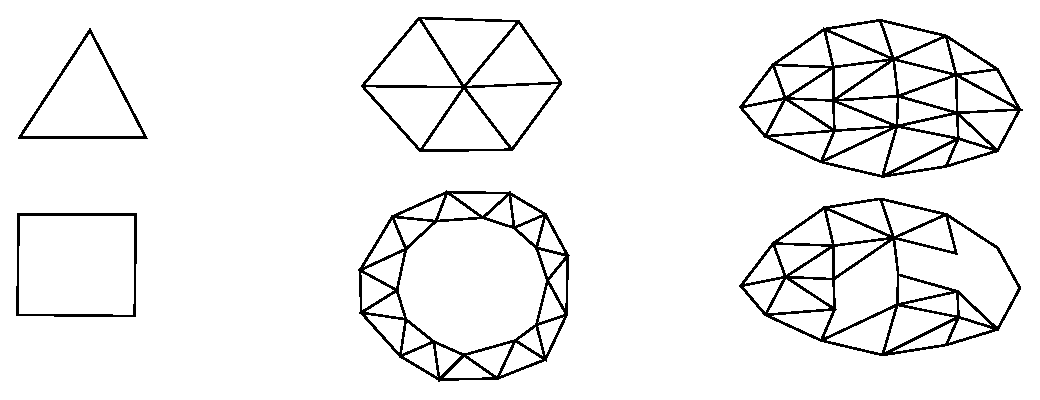
\includegraphics[scale=0.4]{SCGraphs.eps}
\end{figure}
\pause

\begin{block}{New Problem}
{Estimate $diam(G)$, in terms of $\vert G \vert$, where $G$ is a finite Cayley graph with the triangle patch property.
 }
\end{block}

\end{frame}
%-------------------------------------------------------------------------




\begin{frame}\frametitle{}



\begin{block}{Proposition (Z, 2017)}
{Let $G$ be a Cayley graph with the triangle patch property. Then 
\begin{center}
$diam(G) \leq 2 \sqrt{\vert G \vert}.$
\end{center}

 }
\end{block}
\begin{block}{Corollary}
{For an $m$ sheeted universal cover $\hat{X}$ of a compact length space $X$ with $diam(X)=1$

$$diam (\hat{X}) \leq 4 \sqrt{m}+2. $$
 }
 \end{block}



\end{frame}
%-------------------------------------------------------------------------




\begin{frame}\frametitle{}



\begin{block}{Theorem (Benjamini, Finucane, Tessera, 2012)}
{If $\{  G_n \}_{n \in \mathbb{N}}$ is a sequence of Cayley graphs with the triangle patch property and $diam(G_n) \rightarrow \infty$, then
\begin{center}
$diam (G_n) = o( \vert G_n \vert ^p ) $ for any $p>0$.
\end{center}
 
 }
\end{block}


\pause



\begin{block}{Theorem (Benjamini, Finucane, Tessera, 2012)}
{If $\{  G_n \}_{n \in \mathbb{N}}$ is a sequence of Cayley graphs with $diam(G_n) \rightarrow \infty$
\begin{center}
and $ \vert G_n \vert = O(   diam (G_n)^q ) $ for some $q>0,$
\end{center} then there is a subsequence which after scaling, converges to a torus of dimension $\leq q$ in the Gromov-Hausdorff sense.
 }
\end{block}


\end{frame}

%-------------------------------------------------------------------------


\begin{frame}\frametitle{}


References\\

\bigskip

https://mathoverflow.net/questions/7732/diameter-of-m-fold-cover.\\

\bigskip

https://mathoverflow.net/questions/8534/diameter-of-universal-cover\\

\bigskip

I. Benjamini, H. Finucane and R. Tessera. On the scaling limit of finite vertex transitive graphs with large diameter. arXiv:1203.5624.

\end{frame}

%----------------------------------------------------------------

\end{document}


